\begin{figure}[htbp]
\centering
\resizebox{\textwidth}{!}{%
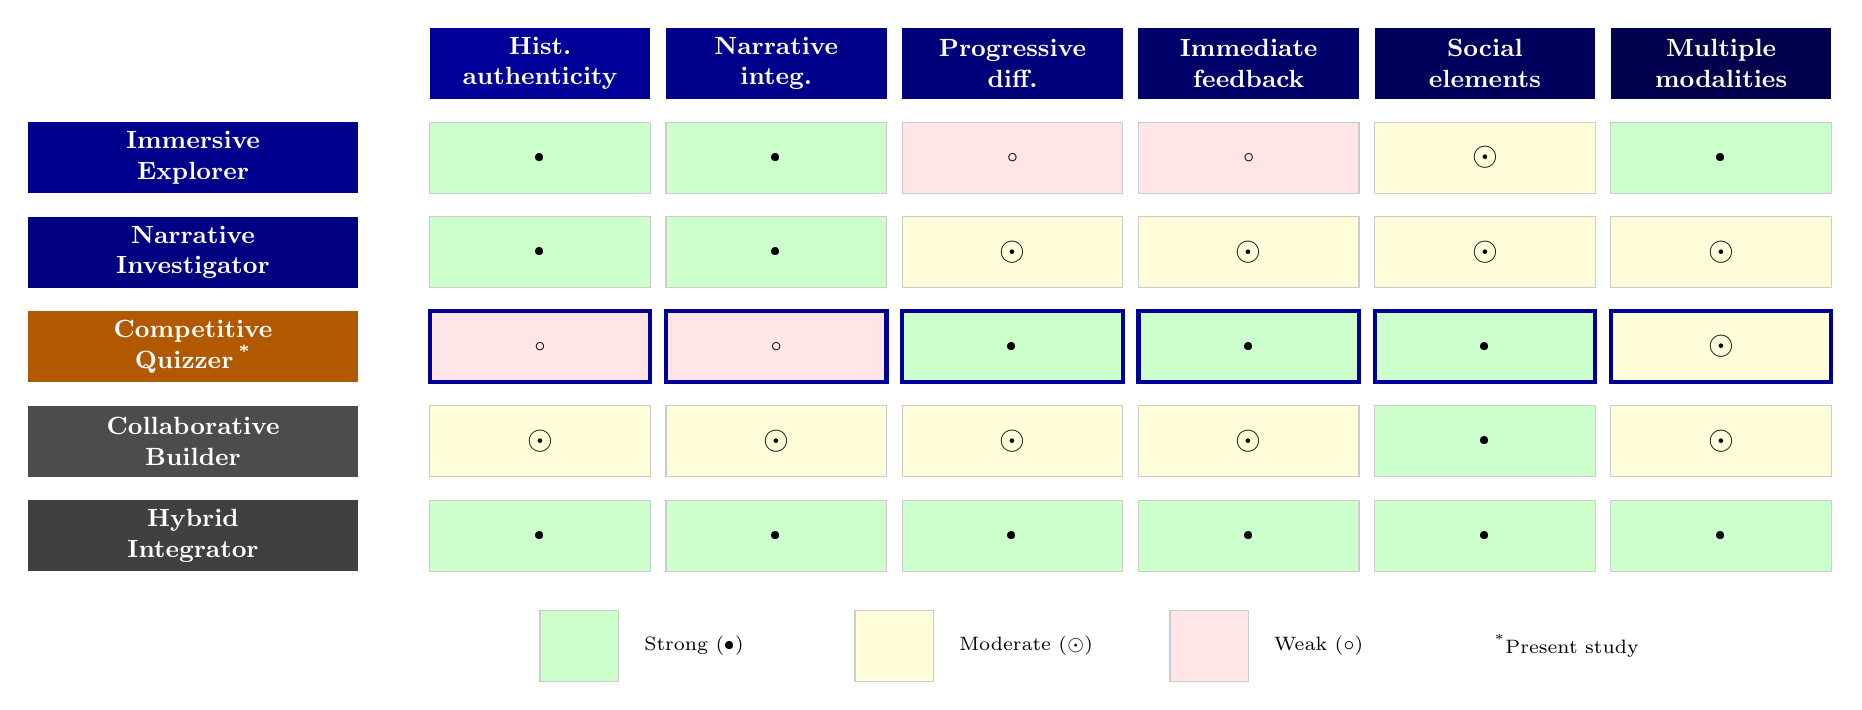
\begin{tikzpicture}[
  hdr/.style={font=\small\bfseries, text=white, minimum height=0.9cm,
    minimum width=2.8cm, align=center},
  rhdr/.style={font=\small\bfseries, text=white, minimum height=0.9cm,
    minimum width=4.2cm, align=center, anchor=east},
  cell/.style={rectangle, draw=gray!40, minimum height=0.9cm,
    minimum width=2.8cm, align=center, font=\scriptsize},
  strong/.style={cell, fill=green!20},
  moderate/.style={cell, fill=yellow!15},
  weak/.style={cell, fill=red!10},
  highlight/.style={draw=blue!60!black, line width=1.5pt},
]

% Column headers
\node[hdr, fill=blue!60!black] at (0, 0) {Hist.\\authenticity};
\node[hdr, fill=blue!54!black] at (3.0, 0) {Narrative\\integ.};
\node[hdr, fill=blue!48!black] at (6.0, 0) {Progressive\\diff.};
\node[hdr, fill=blue!42!black] at (9.0, 0) {Immediate\\feedback};
\node[hdr, fill=blue!36!black] at (12.0, 0) {Social\\elements};
\node[hdr, fill=blue!30!black] at (15.0, 0) {Multiple\\modalities};

% Row 1: Immersive Explorer
\node[rhdr, fill=blue!55!black] at (-2.3, -1.2) {Immersive\\Explorer};
\node[strong] at (0, -1.2) {\textbullet};
\node[strong] at (3.0, -1.2) {\textbullet};
\node[weak] at (6.0, -1.2) {$\circ$};
\node[weak] at (9.0, -1.2) {$\circ$};
\node[moderate] at (12.0, -1.2) {\large$\odot$};
\node[strong] at (15.0, -1.2) {\textbullet};

% Row 2: Narrative Investigator
\node[rhdr, fill=blue!50!black] at (-2.3, -2.4) {Narrative\\Investigator};
\node[strong] at (0, -2.4) {\textbullet};
\node[strong] at (3.0, -2.4) {\textbullet};
\node[moderate] at (6.0, -2.4) {\large$\odot$};
\node[moderate] at (9.0, -2.4) {\large$\odot$};
\node[moderate] at (12.0, -2.4) {\large$\odot$};
\node[moderate] at (15.0, -2.4) {\large$\odot$};

% Row 3: Competitive Quizzer (highlighted — present study)
\node[rhdr, fill=orange!70!black] at (-2.3, -3.6) {Competitive\\Quizzer\,\textsuperscript{*}};
\node[weak, highlight] at (0, -3.6) {$\circ$};
\node[weak, highlight] at (3.0, -3.6) {$\circ$};
\node[strong, highlight] at (6.0, -3.6) {\textbullet};
\node[strong, highlight] at (9.0, -3.6) {\textbullet};
\node[strong, highlight] at (12.0, -3.6) {\textbullet};
\node[moderate, highlight] at (15.0, -3.6) {\large$\odot$};

% Row 4: Collaborative Builder
\node[rhdr, fill=gray!60!black] at (-2.3, -4.8) {Collaborative\\Builder};
\node[moderate] at (0, -4.8) {\large$\odot$};
\node[moderate] at (3.0, -4.8) {\large$\odot$};
\node[moderate] at (6.0, -4.8) {\large$\odot$};
\node[moderate] at (9.0, -4.8) {\large$\odot$};
\node[strong] at (12.0, -4.8) {\textbullet};
\node[moderate] at (15.0, -4.8) {\large$\odot$};

% Row 5: Hybrid Integrator
\node[rhdr, fill=gray!50!black] at (-2.3, -6.0) {Hybrid\\Integrator};
\node[strong] at (0, -6.0) {\textbullet};
\node[strong] at (3.0, -6.0) {\textbullet};
\node[strong] at (6.0, -6.0) {\textbullet};
\node[strong] at (9.0, -6.0) {\textbullet};
\node[strong] at (12.0, -6.0) {\textbullet};
\node[strong] at (15.0, -6.0) {\textbullet};

% Legend
\node[strong, minimum width=1.0cm] at (0.5, -7.4) {};
\node[font=\scriptsize, anchor=west] at (1.2, -7.4) {Strong (\textbullet)};
\node[moderate, minimum width=1.0cm] at (4.5, -7.4) {};
\node[font=\scriptsize, anchor=west] at (5.2, -7.4) {Moderate ($\odot$)};
\node[weak, minimum width=1.0cm] at (8.5, -7.4) {};
\node[font=\scriptsize, anchor=west] at (9.2, -7.4) {Weak ($\circ$)};
\node[font=\scriptsize, anchor=west] at (12.0, -7.4) {\textsuperscript{*}Present study};

\end{tikzpicture}%
}% end resizebox
\caption{Design principle emphasis across the five implementation archetypes. The Competitive Quizzer (highlighted), selected for the present study, prioritises scalable principles (feedback, progression) while under-implementing history-specific principles (authenticity, narrative).}
\label{fig:principle-archetype-mapping}
\end{figure}
